\documentclass[12pt]{article}
\usepackage{amsmath}
\usepackage{amsfonts}
\usepackage{graphicx}

\title{COMP9417 HomeWork 2}
\author{Ping GAO z5163482}
\date{\today}
\begin{document}
    \maketitle
    \section{Q1}\label{sec:q1}
    \subsection{Part A}\label{subsec:part-a}
    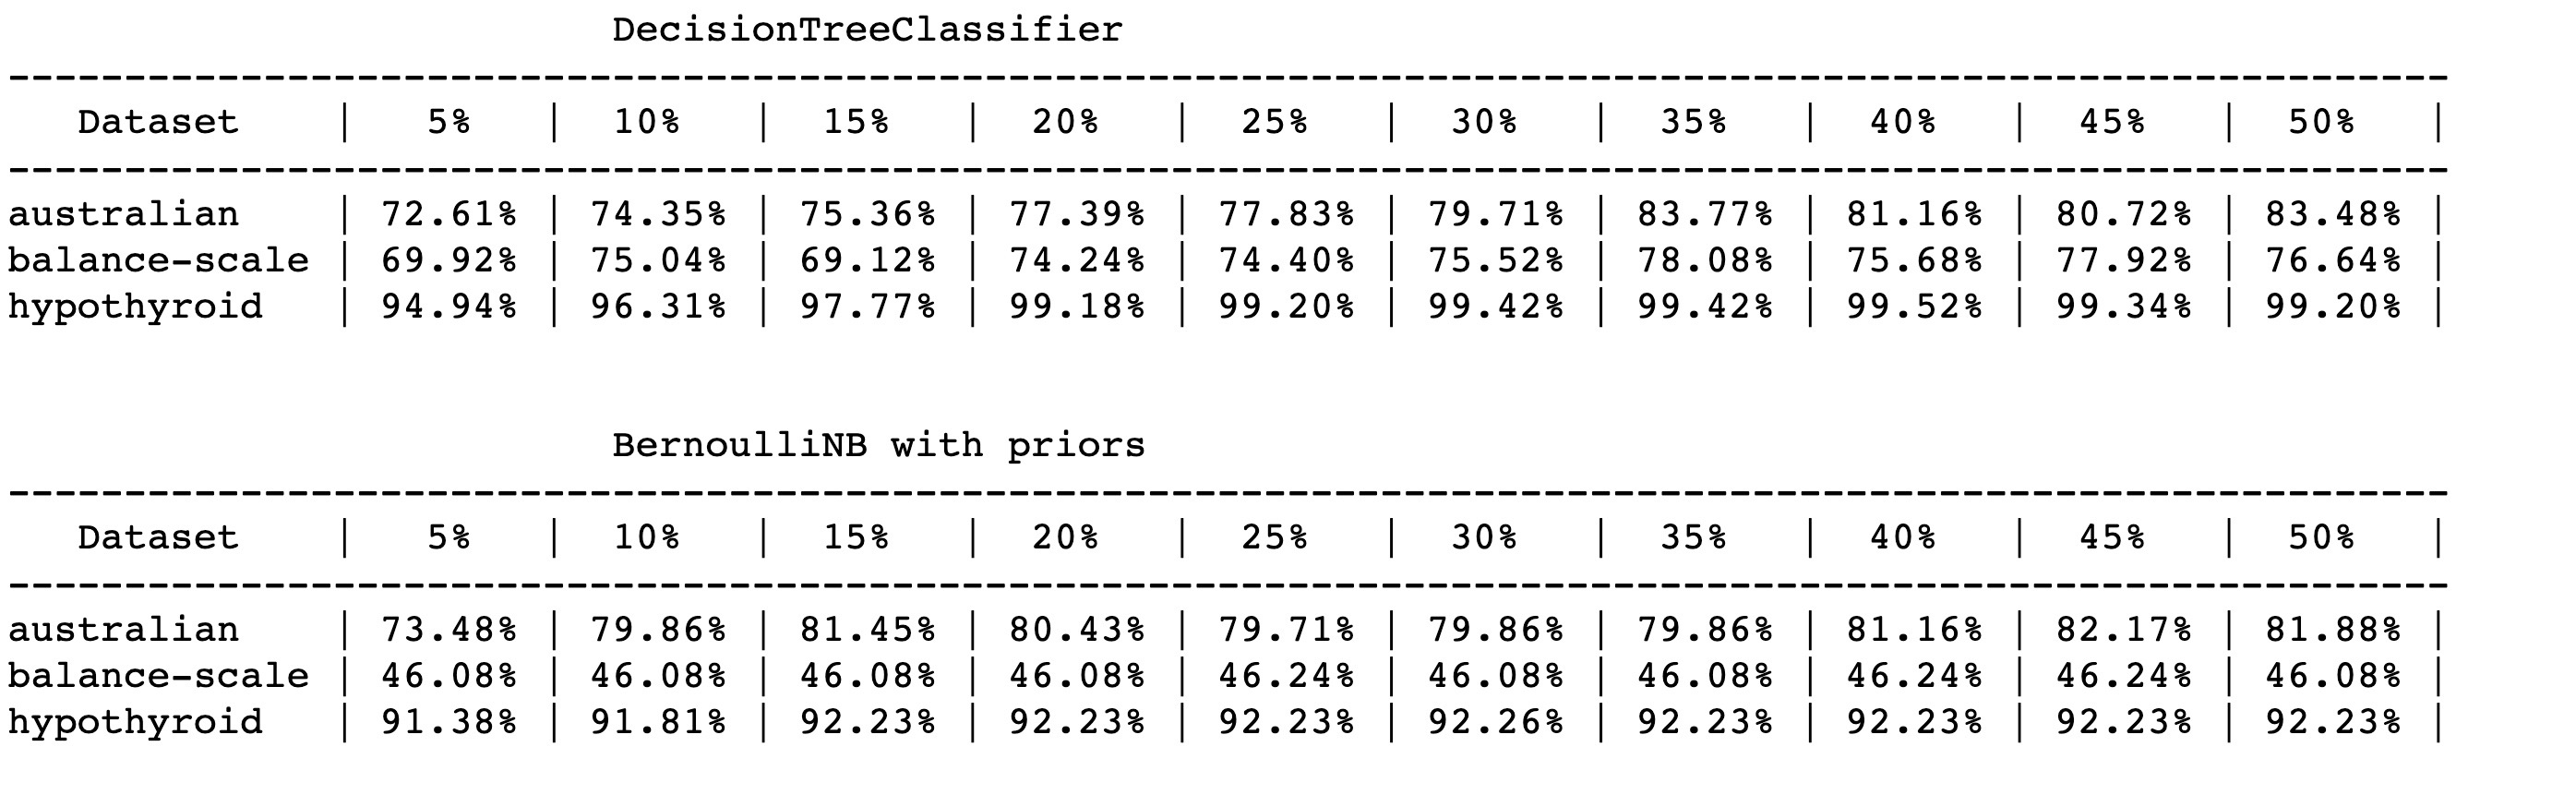
\includegraphics[scale=0.18]{result.jpeg}
    \subsection{Part B}\label{subsec:part-b}
    I think (3), (5) statements are true.
    \subsection{Part C}\label{subsec:part-c}
    I choose (1).
    \section{Q2}\label{sec:q2}
    \subsection{Part A}\label{subsec:part-a2}
    My accuracy score for the test dataset is 82.77\%. \\
    My accuracy score for the training dataset is 85.65\%.
    \subsection{Part B}\label{subsec:part-b2}
    The min\_samples\_leaf number of 5 to 7 give the optimal
    result, this can be observed by compare the auc score in
    the part c's plots, pick the maximum score with the lowest varience.
    \subsection{Part C}\label{subsec:part-c2}
    \begin{center}
        Plot For Test Dataset
    \end{center}
    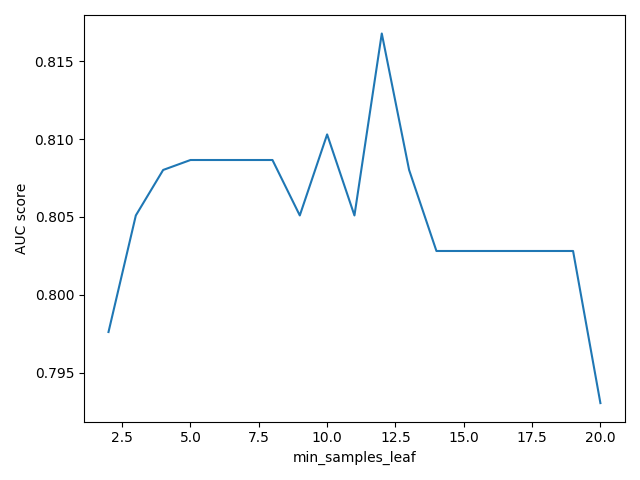
\includegraphics[scale=0.8]{../Plot/plot_test.png}
    \begin{center}
        Plot For Train Dataset
    \end{center}
    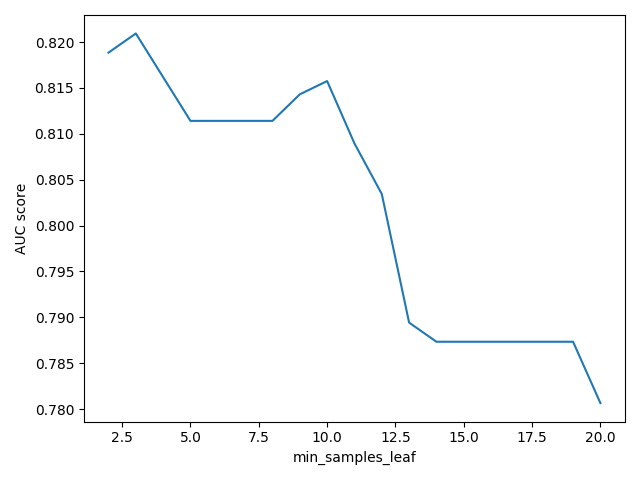
\includegraphics[scale=0.8]{../Plot/plot_train.png}
    \subsection{Part D}\label{subsec:part-d}
    We make the asumption that 'Sex' and 'Pclass' are independent feature. \\
    Thus, {\fontsize{9} P(S=true \lvert G=female,C=1)  = P(S= true \lvert G=female) *
    P(S=true \lvert C=1)} \\
    P(S=true \lvert G=female) = P(G=female) \cap P(S=true) / P(G=female) \\
    = 109 / 573 \\
    P(S=true \lvert C=1) = 136/216 \\
     P(S=true \lvert G=female,C=1) = 11.98\%.


\end{document}